\documentclass[1p]{elsarticle_modified}
%\bibliographystyle{elsarticle-num}

%\usepackage[colorlinks]{hyperref}
%\usepackage{abbrmath_seonhwa} %\Abb, \Ascr, \Acal ,\Abf, \Afrak
\usepackage{amsfonts}
\usepackage{amssymb}
\usepackage{amsmath}
\usepackage{amsthm}
\usepackage{scalefnt}
\usepackage{amsbsy}
\usepackage{kotex}
\usepackage{caption}
\usepackage{subfig}
\usepackage{color}
\usepackage{graphicx}
\usepackage{xcolor} %% white, black, red, green, blue, cyan, magenta, yellow
\usepackage{float}
\usepackage{setspace}
\usepackage{hyperref}

\usepackage{tikz}
\usetikzlibrary{arrows}

\usepackage{multirow}
\usepackage{array} % fixed length table
\usepackage{hhline}

%%%%%%%%%%%%%%%%%%%%%
\makeatletter
\renewcommand*\env@matrix[1][\arraystretch]{%
	\edef\arraystretch{#1}%
	\hskip -\arraycolsep
	\let\@ifnextchar\new@ifnextchar
	\array{*\c@MaxMatrixCols c}}
\makeatother %https://tex.stackexchange.com/questions/14071/how-can-i-increase-the-line-spacing-in-a-matrix
%%%%%%%%%%%%%%%

\usepackage[normalem]{ulem}

\newcommand{\msout}[1]{\ifmmode\text{\sout{\ensuremath{#1}}}\else\sout{#1}\fi}
%SOURCE: \msout is \stkout macro in https://tex.stackexchange.com/questions/20609/strikeout-in-math-mode

\newcommand{\cancel}[1]{
	\ifmmode
	{\color{red}\msout{#1}}
	\else
	{\color{red}\sout{#1}}
	\fi
}

\newcommand{\add}[1]{
	{\color{blue}\uwave{#1}}
}

\newcommand{\replace}[2]{
	\ifmmode
	{\color{red}\msout{#1}}{\color{blue}\uwave{#2}}
	\else
	{\color{red}\sout{#1}}{\color{blue}\uwave{#2}}
	\fi
}

\newcommand{\Sol}{\mathcal{S}} %segment
\newcommand{\D}{D} %diagram
\newcommand{\A}{\mathcal{A}} %arc


%%%%%%%%%%%%%%%%%%%%%%%%%%%%%5 test

\def\sl{\operatorname{\textup{SL}}(2,\Cbb)}
\def\psl{\operatorname{\textup{PSL}}(2,\Cbb)}
\def\quan{\mkern 1mu \triangleright \mkern 1mu}

\theoremstyle{definition}
\newtheorem{thm}{Theorem}[section]
\newtheorem{prop}[thm]{Proposition}
\newtheorem{lem}[thm]{Lemma}
\newtheorem{ques}[thm]{Question}
\newtheorem{cor}[thm]{Corollary}
\newtheorem{defn}[thm]{Definition}
\newtheorem{exam}[thm]{Example}
\newtheorem{rmk}[thm]{Remark}
\newtheorem{alg}[thm]{Algorithm}

\newcommand{\I}{\sqrt{-1}}
\begin{document}

%\begin{frontmatter}
%
%\title{Boundary parabolic representations of knots up to 8 crossings}
%
%%% Group authors per affiliation:
%\author{Yunhi Cho} 
%\address{Department of Mathematics, University of Seoul, Seoul, Korea}
%\ead{yhcho@uos.ac.kr}
%
%
%\author{Seonhwa Kim} %\fnref{s_kim}}
%\address{Center for Geometry and Physics, Institute for Basic Science, Pohang, 37673, Korea}
%\ead{ryeona17@ibs.re.kr}
%
%\author{Hyuk Kim}
%\address{Department of Mathematical Sciences, Seoul National University, Seoul 08826, Korea}
%\ead{hyukkim@snu.ac.kr}
%
%\author{Seokbeom Yoon}
%\address{Department of Mathematical Sciences, Seoul National University, Seoul, 08826,  Korea}
%\ead{sbyoon15@snu.ac.kr}
%
%\begin{abstract}
%We find all boundary parabolic representation of knots up to 8 crossings.
%
%\end{abstract}
%\begin{keyword}
%    \MSC[2010] 57M25 
%\end{keyword}
%
%\end{frontmatter}

%\linenumbers
%\tableofcontents
%
\newcommand\colored[1]{\textcolor{white}{\rule[-0.35ex]{0.8em}{1.4ex}}\kern-0.8em\color{red} #1}%
%\newcommand\colored[1]{\textcolor{white}{ #1}\kern-2.17ex	\textcolor{white}{ #1}\kern-1.81ex	\textcolor{white}{ #1}\kern-2.15ex\color{red}#1	}

{\Large $\underline{12a_{0911}~(K12a_{0911})}$}

\setlength{\tabcolsep}{10pt}
\renewcommand{\arraystretch}{1.6}
\vspace{1cm}\begin{tabular}{m{100pt}>{\centering\arraybackslash}m{274pt}}
\multirow{5}{120pt}{
	\centering
	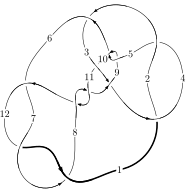
\includegraphics[width=112pt]{../../../GIT/diagram.site/Diagrams/png/1712_12a_0911.png}\\
\ \ \ A knot diagram\footnotemark}&
\allowdisplaybreaks
\textbf{Linearized knot diagam} \\
\cline{2-2}
 &
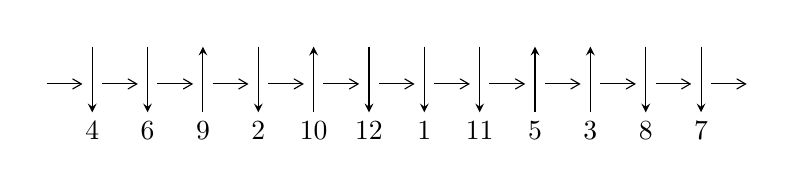
\begin{tikzpicture}[x=20pt, y=17pt]
	% nodes
	\node (C0) at (0, 0) {};
	\node (C1) at (1, 0) {};
	\node (C1U) at (1, +1) {};
	\node (C1D) at (1, -1) {4};

	\node (C2) at (2, 0) {};
	\node (C2U) at (2, +1) {};
	\node (C2D) at (2, -1) {6};

	\node (C3) at (3, 0) {};
	\node (C3U) at (3, +1) {};
	\node (C3D) at (3, -1) {9};

	\node (C4) at (4, 0) {};
	\node (C4U) at (4, +1) {};
	\node (C4D) at (4, -1) {2};

	\node (C5) at (5, 0) {};
	\node (C5U) at (5, +1) {};
	\node (C5D) at (5, -1) {10};

	\node (C6) at (6, 0) {};
	\node (C6U) at (6, +1) {};
	\node (C6D) at (6, -1) {12};

	\node (C7) at (7, 0) {};
	\node (C7U) at (7, +1) {};
	\node (C7D) at (7, -1) {1};

	\node (C8) at (8, 0) {};
	\node (C8U) at (8, +1) {};
	\node (C8D) at (8, -1) {11};

	\node (C9) at (9, 0) {};
	\node (C9U) at (9, +1) {};
	\node (C9D) at (9, -1) {5};

	\node (C10) at (10, 0) {};
	\node (C10U) at (10, +1) {};
	\node (C10D) at (10, -1) {3};

	\node (C11) at (11, 0) {};
	\node (C11U) at (11, +1) {};
	\node (C11D) at (11, -1) {8};

	\node (C12) at (12, 0) {};
	\node (C12U) at (12, +1) {};
	\node (C12D) at (12, -1) {7};
	\node (C13) at (13, 0) {};

	% arrows
	\draw[->,>={angle 60}]
	(C0) edge (C1) (C1) edge (C2) (C2) edge (C3) (C3) edge (C4) (C4) edge (C5) (C5) edge (C6) (C6) edge (C7) (C7) edge (C8) (C8) edge (C9) (C9) edge (C10) (C10) edge (C11) (C11) edge (C12) (C12) edge (C13) ;	\draw[->,>=stealth]
	(C1U) edge (C1D) (C2U) edge (C2D) (C3D) edge (C3U) (C4U) edge (C4D) (C5D) edge (C5U) (C6U) edge (C6D) (C7U) edge (C7D) (C8U) edge (C8D) (C9D) edge (C9U) (C10D) edge (C10U) (C11U) edge (C11D) (C12U) edge (C12D) ;
	\end{tikzpicture} \\
\hhline{~~} \\& 
\textbf{Solving Sequence} \\ \cline{2-2} 
 &
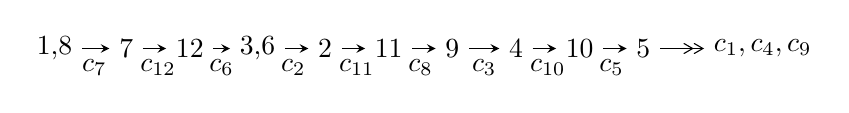
\begin{tikzpicture}[x=23pt, y=7pt]
	% node
	\node (A0) at (-1/8, 0) {1,8};
	\node (A1) at (1, 0) {7};
	\node (A2) at (2, 0) {12};
	\node (A3) at (49/16, 0) {3,6};
	\node (A4) at (33/8, 0) {2};
	\node (A5) at (41/8, 0) {11};
	\node (A6) at (49/8, 0) {9};
	\node (A7) at (57/8, 0) {4};
	\node (A8) at (65/8, 0) {10};
	\node (A9) at (73/8, 0) {5};
	\node (C1) at (1/2, -1) {$c_{7}$};
	\node (C2) at (3/2, -1) {$c_{12}$};
	\node (C3) at (5/2, -1) {$c_{6}$};
	\node (C4) at (29/8, -1) {$c_{2}$};
	\node (C5) at (37/8, -1) {$c_{11}$};
	\node (C6) at (45/8, -1) {$c_{8}$};
	\node (C7) at (53/8, -1) {$c_{3}$};
	\node (C8) at (61/8, -1) {$c_{10}$};
	\node (C9) at (69/8, -1) {$c_{5}$};
	\node (A10) at (11, 0) {$c_{1},c_{4},c_{9}$};

	% edge
	\draw[->,>=stealth]	
	(A0) edge (A1) (A1) edge (A2) (A2) edge (A3) (A3) edge (A4) (A4) edge (A5) (A5) edge (A6) (A6) edge (A7) (A7) edge (A8) (A8) edge (A9) ;
	\draw[->>,>={angle 60}]	
	(A9) edge (A10);
\end{tikzpicture} \\ 

\end{tabular} \\

\footnotetext{
The image of knot diagram is generated by the software ``\textbf{Draw programme}" developed by Andrew Bartholomew(\url{http://www.layer8.co.uk/maths/draw/index.htm\#Running-draw}), where we modified some parts for our purpose(\url{https://github.com/CATsTAILs/LinksPainter}).
}\phantom \\ \newline 
\centering \textbf{Ideals for irreducible components\footnotemark of $X_{\text{par}}$} 
 
\begin{align*}
I^u_{1}&=\langle 
2.55005\times10^{55} u^{99}+1.78130\times10^{55} u^{98}+\cdots+1.02735\times10^{54} b-1.90596\times10^{55},\\
\phantom{I^u_{1}}&\phantom{= \langle  }-2.30960\times10^{54} u^{99}-2.60296\times10^{53} u^{98}+\cdots+1.02735\times10^{54} a+2.71064\times10^{54},\;u^{100}+2 u^{99}+\cdots+u-1\rangle \\
I^u_{2}&=\langle 
2 u^4-2 u^3-7 u^2+7 b-2 u-1,\;6 u^4+8 u^3-7 u^2+7 a-6 u+4,\;u^5+u^4-2 u^3- u^2+u-1\rangle \\
\\
\end{align*}
\raggedright * 2 irreducible components of $\dim_{\mathbb{C}}=0$, with total 105 representations.\\
\footnotetext{All coefficients of polynomials are rational numbers. But the coefficients are sometimes approximated in decimal forms when there is not enough margin.}
\newpage
\renewcommand{\arraystretch}{1}
\centering \section*{I. $I^u_{1}= \langle 2.55\times10^{55} u^{99}+1.78\times10^{55} u^{98}+\cdots+1.03\times10^{54} b-1.91\times10^{55},\;-2.31\times10^{54} u^{99}-2.60\times10^{53} u^{98}+\cdots+1.03\times10^{54} a+2.71\times10^{54},\;u^{100}+2 u^{99}+\cdots+u-1 \rangle$}
\flushleft \textbf{(i) Arc colorings}\\
\begin{tabular}{m{7pt} m{180pt} m{7pt} m{180pt} }
\flushright $a_{1}=$&$\begin{pmatrix}0\\u\end{pmatrix}$ \\
\flushright $a_{8}=$&$\begin{pmatrix}1\\0\end{pmatrix}$ \\
\flushright $a_{7}=$&$\begin{pmatrix}1\\- u^2\end{pmatrix}$ \\
\flushright $a_{12}=$&$\begin{pmatrix}u\\- u^3+u\end{pmatrix}$ \\
\flushright $a_{3}=$&$\begin{pmatrix}2.24811 u^{99}+0.253365 u^{98}+\cdots-0.644151 u-2.63847\\-24.8215 u^{99}-17.3387 u^{98}+\cdots-31.6225 u+18.5521\end{pmatrix}$ \\
\flushright $a_{6}=$&$\begin{pmatrix}- u^2+1\\u^4-2 u^2\end{pmatrix}$ \\
\flushright $a_{2}=$&$\begin{pmatrix}-12.8554 u^{99}-10.3071 u^{98}+\cdots-19.7406 u+8.23996\\-33.1829 u^{99}-22.7159 u^{98}+\cdots-41.6270 u+24.6702\end{pmatrix}$ \\
\flushright $a_{11}=$&$\begin{pmatrix}- u^3+2 u\\- u^3+u\end{pmatrix}$ \\
\flushright $a_{9}=$&$\begin{pmatrix}u^6-3 u^4+2 u^2+1\\u^6-2 u^4+u^2\end{pmatrix}$ \\
\flushright $a_{4}=$&$\begin{pmatrix}-11.4644 u^{99}-9.40616 u^{98}+\cdots-18.1363 u+7.33735\\-43.7815 u^{99}-29.8900 u^{98}+\cdots-57.0219 u+32.7738\end{pmatrix}$ \\
\flushright $a_{10}=$&$\begin{pmatrix}-0.735233 u^{99}-0.0386406 u^{98}+\cdots-3.61695 u+0.645082\\19.0168 u^{99}+13.0073 u^{98}+\cdots+23.4427 u-14.2277\end{pmatrix}$ \\
\flushright $a_{5}=$&$\begin{pmatrix}3.85489 u^{99}+2.47469 u^{98}+\cdots+4.29212 u-2.64226\\-15.8972 u^{99}-10.5712 u^{98}+\cdots-22.7675 u+12.2305\end{pmatrix}$\\&\end{tabular}
\flushleft \textbf{(ii) Obstruction class $= -1$}\\~\\
\flushleft \textbf{(iii) Cusp Shapes $= 76.2668 u^{99}+56.8751 u^{98}+\cdots+75.3902 u-55.1984$}\\~\\
\newpage\renewcommand{\arraystretch}{1}
\flushleft \textbf{(iv) u-Polynomials at the component}\newline \\
\begin{tabular}{m{50pt}|m{274pt}}
Crossings & \hspace{64pt}u-Polynomials at each crossing \\
\hline $$\begin{aligned}c_{1},c_{4}\end{aligned}$$&$\begin{aligned}
&u^{100}-6 u^{99}+\cdots+1149 u-49
\end{aligned}$\\
\hline $$\begin{aligned}c_{2}\end{aligned}$$&$\begin{aligned}
&7(7 u^{100}+35 u^{99}+\cdots+385706 u-40879)
\end{aligned}$\\
\hline $$\begin{aligned}c_{3}\end{aligned}$$&$\begin{aligned}
&7(7 u^{100}-147 u^{99}+\cdots-311196 u-14099)
\end{aligned}$\\
\hline $$\begin{aligned}c_{5},c_{9}\end{aligned}$$&$\begin{aligned}
&u^{100}+2 u^{99}+\cdots+5 u+1
\end{aligned}$\\
\hline $$\begin{aligned}c_{6},c_{7},c_{12}\end{aligned}$$&$\begin{aligned}
&u^{100}+2 u^{99}+\cdots+u-1
\end{aligned}$\\
\hline $$\begin{aligned}c_{8},c_{11}\end{aligned}$$&$\begin{aligned}
&u^{100}-6 u^{99}+\cdots+25745 u-4025
\end{aligned}$\\
\hline $$\begin{aligned}c_{10}\end{aligned}$$&$\begin{aligned}
&u^{100}+3 u^{99}+\cdots+17472 u+1568
\end{aligned}$\\
\hline
\end{tabular}\\~\\
\newpage\renewcommand{\arraystretch}{1}
\flushleft \textbf{(v) Riley Polynomials at the component}\newline \\
\begin{tabular}{m{50pt}|m{274pt}}
Crossings & \hspace{64pt}Riley Polynomials at each crossing \\
\hline $$\begin{aligned}c_{1},c_{4}\end{aligned}$$&$\begin{aligned}
&y^{100}-54 y^{99}+\cdots-355685 y+2401
\end{aligned}$\\
\hline $$\begin{aligned}c_{2}\end{aligned}$$&$\begin{aligned}
&49(49 y^{100}-12187 y^{99}+\cdots-3.62058\times10^{10} y+1.67109\times10^{9})
\end{aligned}$\\
\hline $$\begin{aligned}c_{3}\end{aligned}$$&$\begin{aligned}
&49(49 y^{100}-14049 y^{99}+\cdots-6.34678\times10^{10} y+1.98782\times10^{8})
\end{aligned}$\\
\hline $$\begin{aligned}c_{5},c_{9}\end{aligned}$$&$\begin{aligned}
&y^{100}-54 y^{99}+\cdots-7 y+1
\end{aligned}$\\
\hline $$\begin{aligned}c_{6},c_{7},c_{12}\end{aligned}$$&$\begin{aligned}
&y^{100}-82 y^{99}+\cdots-7 y+1
\end{aligned}$\\
\hline $$\begin{aligned}c_{8},c_{11}\end{aligned}$$&$\begin{aligned}
&y^{100}+70 y^{99}+\cdots-361276175 y+16200625
\end{aligned}$\\
\hline $$\begin{aligned}c_{10}\end{aligned}$$&$\begin{aligned}
&y^{100}-33 y^{99}+\cdots-259083776 y+2458624
\end{aligned}$\\
\hline
\end{tabular}\\~\\
\newpage\flushleft \textbf{(vi) Complex Volumes and Cusp Shapes}
$$\begin{array}{c|c|c}  
\text{Solutions to }I^u_{1}& \I (\text{vol} + \sqrt{-1}CS) & \text{Cusp shape}\\
 \hline 
\begin{aligned}
u &= \phantom{-}0.066180 + 0.860765 I \\
a &= \phantom{-}0.87155 - 2.12153 I \\
b &= \phantom{-}0.61301 - 1.78801 I\end{aligned}
 & \phantom{-}7.76831 + 1.78382 I & \phantom{-0.000000 } 0 \\ \hline\begin{aligned}
u &= \phantom{-}0.066180 - 0.860765 I \\
a &= \phantom{-}0.87155 + 2.12153 I \\
b &= \phantom{-}0.61301 + 1.78801 I\end{aligned}
 & \phantom{-}7.76831 - 1.78382 I & \phantom{-0.000000 } 0 \\ \hline\begin{aligned}
u &= \phantom{-}0.125303 + 0.844813 I \\
a &= \phantom{-}0.00052 + 3.24559 I \\
b &= \phantom{-}0.34459 + 2.71163 I\end{aligned}
 & \phantom{-}5.8756 - 13.5209 I & \phantom{-0.000000 } 0 \\ \hline\begin{aligned}
u &= \phantom{-}0.125303 - 0.844813 I \\
a &= \phantom{-}0.00052 - 3.24559 I \\
b &= \phantom{-}0.34459 - 2.71163 I\end{aligned}
 & \phantom{-}5.8756 + 13.5209 I & \phantom{-0.000000 } 0 \\ \hline\begin{aligned}
u &= -0.135762 + 0.841793 I \\
a &= -0.00022 + 2.29080 I \\
b &= -0.26671 + 1.96639 I\end{aligned}
 & \phantom{-}2.30679 + 7.72312 I & \phantom{-0.000000 } 0 \\ \hline\begin{aligned}
u &= -0.135762 - 0.841793 I \\
a &= -0.00022 - 2.29080 I \\
b &= -0.26671 - 1.96639 I\end{aligned}
 & \phantom{-}2.30679 - 7.72312 I & \phantom{-0.000000 } 0 \\ \hline\begin{aligned}
u &= \phantom{-}0.084808 + 0.824876 I \\
a &= -0.25875 - 3.34323 I \\
b &= -0.49311 - 2.87868 I\end{aligned}
 & \phantom{-}8.93550 - 6.71171 I & \phantom{-0.000000 -}0. + 5.58180 I \\ \hline\begin{aligned}
u &= \phantom{-}0.084808 - 0.824876 I \\
a &= -0.25875 + 3.34323 I \\
b &= -0.49311 + 2.87868 I\end{aligned}
 & \phantom{-}8.93550 + 6.71171 I & \phantom{-0.000000 } 0. - 5.58180 I \\ \hline\begin{aligned}
u &= \phantom{-}1.118570 + 0.355935 I \\
a &= -0.411676 + 1.064340 I \\
b &= \phantom{-}1.17459 + 1.01033 I\end{aligned}
 & \phantom{-}4.54352 - 1.52298 I & \phantom{-0.000000 } 0 \\ \hline\begin{aligned}
u &= \phantom{-}1.118570 - 0.355935 I \\
a &= -0.411676 - 1.064340 I \\
b &= \phantom{-}1.17459 - 1.01033 I\end{aligned}
 & \phantom{-}4.54352 + 1.52298 I & \phantom{-0.000000 } 0\\
 \hline 
 \end{array}$$\newpage$$\begin{array}{c|c|c}  
\text{Solutions to }I^u_{1}& \I (\text{vol} + \sqrt{-1}CS) & \text{Cusp shape}\\
 \hline 
\begin{aligned}
u &= -0.063459 + 0.823553 I \\
a &= \phantom{-}0.01587 - 2.41880 I \\
b &= \phantom{-}0.28053 - 1.98760 I\end{aligned}
 & \phantom{-}5.17789 + 2.75522 I & \phantom{-0.000000 } 0 \\ \hline\begin{aligned}
u &= -0.063459 - 0.823553 I \\
a &= \phantom{-}0.01587 + 2.41880 I \\
b &= \phantom{-}0.28053 + 1.98760 I\end{aligned}
 & \phantom{-}5.17789 - 2.75522 I & \phantom{-0.000000 } 0 \\ \hline\begin{aligned}
u &= \phantom{-}0.133069 + 0.812087 I \\
a &= -1.17414 + 1.37179 I \\
b &= -0.71986 + 1.37933 I\end{aligned}
 & \phantom{-}7.53948 - 2.72894 I & \phantom{-0.000000 -}0. + 4.33750 I \\ \hline\begin{aligned}
u &= \phantom{-}0.133069 - 0.812087 I \\
a &= -1.17414 - 1.37179 I \\
b &= -0.71986 - 1.37933 I\end{aligned}
 & \phantom{-}7.53948 + 2.72894 I & \phantom{-0.000000 } 0. - 4.33750 I \\ \hline\begin{aligned}
u &= -1.108750 + 0.404553 I \\
a &= \phantom{-}1.233170 + 0.565323 I \\
b &= -0.21427 + 1.54803 I\end{aligned}
 & -0.67251 - 3.23097 I & \phantom{-0.000000 } 0 \\ \hline\begin{aligned}
u &= -1.108750 - 0.404553 I \\
a &= \phantom{-}1.233170 - 0.565323 I \\
b &= -0.21427 - 1.54803 I\end{aligned}
 & -0.67251 + 3.23097 I & \phantom{-0.000000 } 0 \\ \hline\begin{aligned}
u &= \phantom{-}1.127540 + 0.406548 I \\
a &= -1.80128 + 0.82756 I \\
b &= \phantom{-}0.19262 + 2.25353 I\end{aligned}
 & \phantom{-}2.80795 + 9.01655 I & \phantom{-0.000000 } 0 \\ \hline\begin{aligned}
u &= \phantom{-}1.127540 - 0.406548 I \\
a &= -1.80128 - 0.82756 I \\
b &= \phantom{-}0.19262 - 2.25353 I\end{aligned}
 & \phantom{-}2.80795 - 9.01655 I & \phantom{-0.000000 } 0 \\ \hline\begin{aligned}
u &= -1.20312\phantom{ +0.000000I} \\
a &= \phantom{-}0.236367\phantom{ +0.000000I} \\
b &= -0.701550\phantom{ +0.000000I}\end{aligned}
 & -2.51628\phantom{ +0.000000I} & \phantom{-0.000000 } 0 \\ \hline\begin{aligned}
u &= -0.026000 + 0.786577 I \\
a &= -4.29155 - 2.82581 I \\
b &= -2.37520 - 1.76189 I\end{aligned}
 & \phantom{-}4.40963 + 0.13433 I & -4.43140 + 2.83159 I\\
 \hline 
 \end{array}$$\newpage$$\begin{array}{c|c|c}  
\text{Solutions to }I^u_{1}& \I (\text{vol} + \sqrt{-1}CS) & \text{Cusp shape}\\
 \hline 
\begin{aligned}
u &= -0.026000 - 0.786577 I \\
a &= -4.29155 + 2.82581 I \\
b &= -2.37520 + 1.76189 I\end{aligned}
 & \phantom{-}4.40963 - 0.13433 I & -4.43140 - 2.83159 I \\ \hline\begin{aligned}
u &= -0.072981 + 0.768562 I \\
a &= \phantom{-}1.287060 + 0.166439 I \\
b &= \phantom{-}1.65682 + 0.13967 I\end{aligned}
 & \phantom{-}2.78890 + 4.95396 I & -0.93576 - 7.70957 I \\ \hline\begin{aligned}
u &= -0.072981 - 0.768562 I \\
a &= \phantom{-}1.287060 - 0.166439 I \\
b &= \phantom{-}1.65682 - 0.13967 I\end{aligned}
 & \phantom{-}2.78890 - 4.95396 I & -0.93576 + 7.70957 I \\ \hline\begin{aligned}
u &= -0.603154 + 0.480578 I \\
a &= \phantom{-}0.531251 + 0.247738 I \\
b &= -0.116625 - 0.232744 I\end{aligned}
 & -2.41423 + 3.09068 I & -4.65212 - 8.27933 I \\ \hline\begin{aligned}
u &= -0.603154 - 0.480578 I \\
a &= \phantom{-}0.531251 - 0.247738 I \\
b &= -0.116625 + 0.232744 I\end{aligned}
 & -2.41423 - 3.09068 I & -4.65212 + 8.27933 I \\ \hline\begin{aligned}
u &= \phantom{-}1.179710 + 0.372781 I \\
a &= \phantom{-}1.87644 - 0.67092 I \\
b &= -0.29893 - 2.56412 I\end{aligned}
 & \phantom{-}5.58223 + 2.39089 I & \phantom{-0.000000 } 0 \\ \hline\begin{aligned}
u &= \phantom{-}1.179710 - 0.372781 I \\
a &= \phantom{-}1.87644 + 0.67092 I \\
b &= -0.29893 + 2.56412 I\end{aligned}
 & \phantom{-}5.58223 - 2.39089 I & \phantom{-0.000000 } 0 \\ \hline\begin{aligned}
u &= -1.208580 + 0.298352 I \\
a &= \phantom{-}0.138130 + 0.798805 I \\
b &= -1.39785 - 0.70786 I\end{aligned}
 & -0.659627 - 1.083600 I & \phantom{-0.000000 } 0 \\ \hline\begin{aligned}
u &= -1.208580 - 0.298352 I \\
a &= \phantom{-}0.138130 - 0.798805 I \\
b &= -1.39785 + 0.70786 I\end{aligned}
 & -0.659627 + 1.083600 I & \phantom{-0.000000 } 0 \\ \hline\begin{aligned}
u &= -0.368759 + 0.658434 I \\
a &= -0.200364 + 0.148708 I \\
b &= \phantom{-}0.192399 + 0.236039 I\end{aligned}
 & -1.61628 + 0.90792 I & \phantom{-}0.73056 + 3.87410 I\\
 \hline 
 \end{array}$$\newpage$$\begin{array}{c|c|c}  
\text{Solutions to }I^u_{1}& \I (\text{vol} + \sqrt{-1}CS) & \text{Cusp shape}\\
 \hline 
\begin{aligned}
u &= -0.368759 - 0.658434 I \\
a &= -0.200364 - 0.148708 I \\
b &= \phantom{-}0.192399 - 0.236039 I\end{aligned}
 & -1.61628 - 0.90792 I & \phantom{-}0.73056 - 3.87410 I \\ \hline\begin{aligned}
u &= \phantom{-}0.046166 + 0.753218 I \\
a &= \phantom{-}0.29339 + 1.60136 I \\
b &= -0.337923 + 1.301070 I\end{aligned}
 & \phantom{-}1.06739 - 1.59292 I & -4.21907 + 0.71852 I \\ \hline\begin{aligned}
u &= \phantom{-}0.046166 - 0.753218 I \\
a &= \phantom{-}0.29339 - 1.60136 I \\
b &= -0.337923 - 1.301070 I\end{aligned}
 & \phantom{-}1.06739 + 1.59292 I & -4.21907 - 0.71852 I \\ \hline\begin{aligned}
u &= -1.207020 + 0.373783 I \\
a &= -1.187900 - 0.686360 I \\
b &= \phantom{-}0.29346 - 1.83954 I\end{aligned}
 & \phantom{-}1.66457 + 1.55604 I & \phantom{-0.000000 } 0 \\ \hline\begin{aligned}
u &= -1.207020 - 0.373783 I \\
a &= -1.187900 + 0.686360 I \\
b &= \phantom{-}0.29346 + 1.83954 I\end{aligned}
 & \phantom{-}1.66457 - 1.55604 I & \phantom{-0.000000 } 0 \\ \hline\begin{aligned}
u &= \phantom{-}1.26388\phantom{ +0.000000I} \\
a &= -10.1850\phantom{ +0.000000I} \\
b &= \phantom{-}15.3307\phantom{ +0.000000I}\end{aligned}
 & -3.96123\phantom{ +0.000000I} & \phantom{-0.000000 } 0 \\ \hline\begin{aligned}
u &= \phantom{-}1.199860 + 0.413091 I \\
a &= \phantom{-}0.88673 - 1.23671 I \\
b &= -0.98804 - 1.51467 I\end{aligned}
 & \phantom{-}4.27981 - 6.34812 I & \phantom{-0.000000 } 0 \\ \hline\begin{aligned}
u &= \phantom{-}1.199860 - 0.413091 I \\
a &= \phantom{-}0.88673 + 1.23671 I \\
b &= -0.98804 + 1.51467 I\end{aligned}
 & \phantom{-}4.27981 + 6.34812 I & \phantom{-0.000000 } 0 \\ \hline\begin{aligned}
u &= \phantom{-}0.535734 + 0.490182 I \\
a &= -0.857560 + 0.337611 I \\
b &= \phantom{-}0.035042 - 0.510932 I\end{aligned}
 & \phantom{-}0.80071 - 9.15581 I & -3.31075 + 8.99009 I \\ \hline\begin{aligned}
u &= \phantom{-}0.535734 - 0.490182 I \\
a &= -0.857560 - 0.337611 I \\
b &= \phantom{-}0.035042 + 0.510932 I\end{aligned}
 & \phantom{-}0.80071 + 9.15581 I & -3.31075 - 8.99009 I\\
 \hline 
 \end{array}$$\newpage$$\begin{array}{c|c|c}  
\text{Solutions to }I^u_{1}& \I (\text{vol} + \sqrt{-1}CS) & \text{Cusp shape}\\
 \hline 
\begin{aligned}
u &= \phantom{-}0.026695 + 0.718976 I \\
a &= -0.03361 + 3.09163 I \\
b &= -0.29804 + 2.61186 I\end{aligned}
 & \phantom{-}0.46493 - 1.57636 I & -3.62391 + 3.74056 I \\ \hline\begin{aligned}
u &= \phantom{-}0.026695 - 0.718976 I \\
a &= -0.03361 - 3.09163 I \\
b &= -0.29804 - 2.61186 I\end{aligned}
 & \phantom{-}0.46493 + 1.57636 I & -3.62391 - 3.74056 I \\ \hline\begin{aligned}
u &= \phantom{-}1.244710 + 0.302263 I \\
a &= -1.125240 + 0.246242 I \\
b &= \phantom{-}0.684228 + 0.684322 I\end{aligned}
 & -2.61355 - 2.20912 I & \phantom{-0.000000 } 0 \\ \hline\begin{aligned}
u &= \phantom{-}1.244710 - 0.302263 I \\
a &= -1.125240 - 0.246242 I \\
b &= \phantom{-}0.684228 - 0.684322 I\end{aligned}
 & -2.61355 + 2.20912 I & \phantom{-0.000000 } 0 \\ \hline\begin{aligned}
u &= \phantom{-}0.425289 + 0.569271 I \\
a &= \phantom{-}0.679374 + 0.345318 I \\
b &= -0.322505 + 0.245223 I\end{aligned}
 & \phantom{-}1.16837 + 5.35171 I & -2.33945 - 3.24419 I \\ \hline\begin{aligned}
u &= \phantom{-}0.425289 - 0.569271 I \\
a &= \phantom{-}0.679374 - 0.345318 I \\
b &= -0.322505 - 0.245223 I\end{aligned}
 & \phantom{-}1.16837 - 5.35171 I & -2.33945 + 3.24419 I \\ \hline\begin{aligned}
u &= -1.247730 + 0.335150 I \\
a &= \phantom{-}0.14268 - 2.59678 I \\
b &= \phantom{-}1.90497 - 1.37567 I\end{aligned}
 & \phantom{-}0.63837 + 3.90975 I & \phantom{-0.000000 } 0 \\ \hline\begin{aligned}
u &= -1.247730 - 0.335150 I \\
a &= \phantom{-}0.14268 + 2.59678 I \\
b &= \phantom{-}1.90497 + 1.37567 I\end{aligned}
 & \phantom{-}0.63837 - 3.90975 I & \phantom{-0.000000 } 0 \\ \hline\begin{aligned}
u &= \phantom{-}1.302980 + 0.076339 I \\
a &= -0.177078 - 0.842270 I \\
b &= \phantom{-}0.451240 + 0.097844 I\end{aligned}
 & -4.78110 - 2.15974 I & \phantom{-0.000000 } 0 \\ \hline\begin{aligned}
u &= \phantom{-}1.302980 - 0.076339 I \\
a &= -0.177078 + 0.842270 I \\
b &= \phantom{-}0.451240 - 0.097844 I\end{aligned}
 & -4.78110 + 2.15974 I & \phantom{-0.000000 } 0\\
 \hline 
 \end{array}$$\newpage$$\begin{array}{c|c|c}  
\text{Solutions to }I^u_{1}& \I (\text{vol} + \sqrt{-1}CS) & \text{Cusp shape}\\
 \hline 
\begin{aligned}
u &= \phantom{-}1.276810 + 0.291243 I \\
a &= -1.64166 + 0.89025 I \\
b &= \phantom{-}1.52030 + 2.34735 I\end{aligned}
 & -3.42645 - 2.04331 I & \phantom{-0.000000 } 0 \\ \hline\begin{aligned}
u &= \phantom{-}1.276810 - 0.291243 I \\
a &= -1.64166 - 0.89025 I \\
b &= \phantom{-}1.52030 - 2.34735 I\end{aligned}
 & -3.42645 + 2.04331 I & \phantom{-0.000000 } 0 \\ \hline\begin{aligned}
u &= -1.31785\phantom{ +0.000000I} \\
a &= \phantom{-}0.616471\phantom{ +0.000000I} \\
b &= -0.733009\phantom{ +0.000000I}\end{aligned}
 & -2.21898\phantom{ +0.000000I} & \phantom{-0.000000 } 0 \\ \hline\begin{aligned}
u &= -1.329660 + 0.009805 I \\
a &= \phantom{-}0.667787 - 0.376017 I \\
b &= \phantom{-}1.83737 - 0.03557 I\end{aligned}
 & -7.24915 + 0.12420 I & \phantom{-0.000000 } 0 \\ \hline\begin{aligned}
u &= -1.329660 - 0.009805 I \\
a &= \phantom{-}0.667787 + 0.376017 I \\
b &= \phantom{-}1.83737 + 0.03557 I\end{aligned}
 & -7.24915 - 0.12420 I & \phantom{-0.000000 } 0 \\ \hline\begin{aligned}
u &= \phantom{-}1.286520 + 0.342616 I \\
a &= \phantom{-}3.62577 + 1.50468 I \\
b &= \phantom{-}3.04784 - 2.13233 I\end{aligned}
 & \phantom{-}0.32064 - 4.20537 I & \phantom{-0.000000 } 0 \\ \hline\begin{aligned}
u &= \phantom{-}1.286520 - 0.342616 I \\
a &= \phantom{-}3.62577 - 1.50468 I \\
b &= \phantom{-}3.04784 + 2.13233 I\end{aligned}
 & \phantom{-}0.32064 + 4.20537 I & \phantom{-0.000000 } 0 \\ \hline\begin{aligned}
u &= -1.295980 + 0.307916 I \\
a &= \phantom{-}1.52481 + 0.84597 I \\
b &= -0.74775 + 3.02913 I\end{aligned}
 & -3.68022 + 5.30134 I & \phantom{-0.000000 } 0 \\ \hline\begin{aligned}
u &= -1.295980 - 0.307916 I \\
a &= \phantom{-}1.52481 - 0.84597 I \\
b &= -0.74775 - 3.02913 I\end{aligned}
 & -3.68022 - 5.30134 I & \phantom{-0.000000 } 0 \\ \hline\begin{aligned}
u &= \phantom{-}1.336150 + 0.037532 I \\
a &= -0.668166 - 1.189430 I \\
b &= -0.974750 - 0.539922 I\end{aligned}
 & -6.23871 - 3.34970 I & \phantom{-0.000000 } 0\\
 \hline 
 \end{array}$$\newpage$$\begin{array}{c|c|c}  
\text{Solutions to }I^u_{1}& \I (\text{vol} + \sqrt{-1}CS) & \text{Cusp shape}\\
 \hline 
\begin{aligned}
u &= \phantom{-}1.336150 - 0.037532 I \\
a &= -0.668166 + 1.189430 I \\
b &= -0.974750 + 0.539922 I\end{aligned}
 & -6.23871 + 3.34970 I & \phantom{-0.000000 } 0 \\ \hline\begin{aligned}
u &= -1.334610 + 0.104729 I \\
a &= -0.401638 - 0.914443 I \\
b &= -0.867103 - 0.055077 I\end{aligned}
 & -1.56741 + 5.50751 I & \phantom{-0.000000 } 0 \\ \hline\begin{aligned}
u &= -1.334610 - 0.104729 I \\
a &= -0.401638 + 0.914443 I \\
b &= -0.867103 + 0.055077 I\end{aligned}
 & -1.56741 - 5.50751 I & \phantom{-0.000000 } 0 \\ \hline\begin{aligned}
u &= -1.302260 + 0.324685 I \\
a &= \phantom{-}0.584203 + 0.491239 I \\
b &= -0.02040 + 1.86856 I\end{aligned}
 & -3.15215 + 5.49182 I & \phantom{-0.000000 } 0 \\ \hline\begin{aligned}
u &= -1.302260 - 0.324685 I \\
a &= \phantom{-}0.584203 - 0.491239 I \\
b &= -0.02040 - 1.86856 I\end{aligned}
 & -3.15215 - 5.49182 I & \phantom{-0.000000 } 0 \\ \hline\begin{aligned}
u &= \phantom{-}1.314960 + 0.333665 I \\
a &= -0.223233 - 0.758788 I \\
b &= -1.76656 + 0.86515 I\end{aligned}
 & -1.55939 - 8.93980 I & \phantom{-0.000000 } 0 \\ \hline\begin{aligned}
u &= \phantom{-}1.314960 - 0.333665 I \\
a &= -0.223233 + 0.758788 I \\
b &= -1.76656 - 0.86515 I\end{aligned}
 & -1.55939 + 8.93980 I & \phantom{-0.000000 } 0 \\ \hline\begin{aligned}
u &= \phantom{-}1.312470 + 0.363962 I \\
a &= \phantom{-}1.36690 - 0.90680 I \\
b &= -0.79085 - 1.96456 I\end{aligned}
 & \phantom{-}0.87397 - 7.02667 I & \phantom{-0.000000 } 0 \\ \hline\begin{aligned}
u &= \phantom{-}1.312470 - 0.363962 I \\
a &= \phantom{-}1.36690 + 0.90680 I \\
b &= -0.79085 + 1.96456 I\end{aligned}
 & \phantom{-}0.87397 + 7.02667 I & \phantom{-0.000000 } 0 \\ \hline\begin{aligned}
u &= -1.314330 + 0.390094 I \\
a &= -1.37366 - 0.34309 I \\
b &= -0.22659 - 1.87215 I\end{aligned}
 & \phantom{-}3.45510 + 2.70339 I & \phantom{-0.000000 } 0\\
 \hline 
 \end{array}$$\newpage$$\begin{array}{c|c|c}  
\text{Solutions to }I^u_{1}& \I (\text{vol} + \sqrt{-1}CS) & \text{Cusp shape}\\
 \hline 
\begin{aligned}
u &= -1.314330 - 0.390094 I \\
a &= -1.37366 + 0.34309 I \\
b &= -0.22659 + 1.87215 I\end{aligned}
 & \phantom{-}3.45510 - 2.70339 I & \phantom{-0.000000 } 0 \\ \hline\begin{aligned}
u &= -1.325260 + 0.363911 I \\
a &= -1.78448 - 1.24566 I \\
b &= \phantom{-}1.18856 - 2.94620 I\end{aligned}
 & \phantom{-}4.51646 + 10.99010 I & \phantom{-0.000000 } 0 \\ \hline\begin{aligned}
u &= -1.325260 - 0.363911 I \\
a &= -1.78448 + 1.24566 I \\
b &= \phantom{-}1.18856 + 2.94620 I\end{aligned}
 & \phantom{-}4.51646 - 10.99010 I & \phantom{-0.000000 } 0 \\ \hline\begin{aligned}
u &= -1.37954\phantom{ +0.000000I} \\
a &= \phantom{-}0.525786\phantom{ +0.000000I} \\
b &= -0.307804\phantom{ +0.000000I}\end{aligned}
 & -2.27657\phantom{ +0.000000I} & \phantom{-0.000000 } 0 \\ \hline\begin{aligned}
u &= -1.354270 + 0.350897 I \\
a &= \phantom{-}1.105460 - 0.077103 I \\
b &= \phantom{-}0.31851 + 1.50383 I\end{aligned}
 & \phantom{-}2.85303 + 6.92434 I & \phantom{-0.000000 } 0 \\ \hline\begin{aligned}
u &= -1.354270 - 0.350897 I \\
a &= \phantom{-}1.105460 + 0.077103 I \\
b &= \phantom{-}0.31851 - 1.50383 I\end{aligned}
 & \phantom{-}2.85303 - 6.92434 I & \phantom{-0.000000 } 0 \\ \hline\begin{aligned}
u &= -1.351770 + 0.370394 I \\
a &= \phantom{-}1.77739 + 1.17880 I \\
b &= -0.84705 + 2.89589 I\end{aligned}
 & \phantom{-}1.2299 + 17.8925 I & \phantom{-0.000000 } 0 \\ \hline\begin{aligned}
u &= -1.351770 - 0.370394 I \\
a &= \phantom{-}1.77739 - 1.17880 I \\
b &= -0.84705 - 2.89589 I\end{aligned}
 & \phantom{-}1.2299 - 17.8925 I & \phantom{-0.000000 } 0 \\ \hline\begin{aligned}
u &= \phantom{-}1.356960 + 0.367547 I \\
a &= -1.26141 + 0.86468 I \\
b &= \phantom{-}0.72317 + 2.11532 I\end{aligned}
 & -2.39184 - 12.07600 I & \phantom{-0.000000 } 0 \\ \hline\begin{aligned}
u &= \phantom{-}1.356960 - 0.367547 I \\
a &= -1.26141 - 0.86468 I \\
b &= \phantom{-}0.72317 - 2.11532 I\end{aligned}
 & -2.39184 + 12.07600 I & \phantom{-0.000000 } 0\\
 \hline 
 \end{array}$$\newpage$$\begin{array}{c|c|c}  
\text{Solutions to }I^u_{1}& \I (\text{vol} + \sqrt{-1}CS) & \text{Cusp shape}\\
 \hline 
\begin{aligned}
u &= -1.403610 + 0.172759 I \\
a &= -0.357432 + 0.140146 I \\
b &= \phantom{-}0.045150 + 0.705809 I\end{aligned}
 & -4.64740 - 2.81144 I & \phantom{-0.000000 } 0 \\ \hline\begin{aligned}
u &= -1.403610 - 0.172759 I \\
a &= -0.357432 - 0.140146 I \\
b &= \phantom{-}0.045150 - 0.705809 I\end{aligned}
 & -4.64740 + 2.81144 I & \phantom{-0.000000 } 0 \\ \hline\begin{aligned}
u &= -1.40977 + 0.11256 I \\
a &= \phantom{-}0.350963 + 0.532406 I \\
b &= \phantom{-}0.973998 - 0.537090 I\end{aligned}
 & -5.38865 + 11.04220 I & \phantom{-0.000000 } 0 \\ \hline\begin{aligned}
u &= -1.40977 - 0.11256 I \\
a &= \phantom{-}0.350963 - 0.532406 I \\
b &= \phantom{-}0.973998 + 0.537090 I\end{aligned}
 & -5.38865 - 11.04220 I & \phantom{-0.000000 } 0 \\ \hline\begin{aligned}
u &= \phantom{-}0.467110 + 0.337848 I \\
a &= -0.393316 - 0.183041 I \\
b &= \phantom{-}0.684027 - 0.159400 I\end{aligned}
 & \phantom{-}3.31994 + 0.86651 I & \phantom{-}0.20729 + 2.64307 I \\ \hline\begin{aligned}
u &= \phantom{-}0.467110 - 0.337848 I \\
a &= -0.393316 + 0.183041 I \\
b &= \phantom{-}0.684027 + 0.159400 I\end{aligned}
 & \phantom{-}3.31994 - 0.86651 I & \phantom{-}0.20729 - 2.64307 I \\ \hline\begin{aligned}
u &= \phantom{-}1.42891 + 0.10467 I \\
a &= -0.245132 + 0.379566 I \\
b &= -0.596256 - 0.199428 I\end{aligned}
 & -8.90921 - 4.87685 I & \phantom{-0.000000 } 0 \\ \hline\begin{aligned}
u &= \phantom{-}1.42891 - 0.10467 I \\
a &= -0.245132 - 0.379566 I \\
b &= -0.596256 + 0.199428 I\end{aligned}
 & -8.90921 + 4.87685 I & \phantom{-0.000000 } 0 \\ \hline\begin{aligned}
u &= \phantom{-}0.366259 + 0.423550 I \\
a &= \phantom{-}0.494904 - 1.198700 I \\
b &= -0.184808 + 0.420618 I\end{aligned}
 & \phantom{-}3.66081 - 3.79622 I & \phantom{-}0.61652 + 6.81445 I \\ \hline\begin{aligned}
u &= \phantom{-}0.366259 - 0.423550 I \\
a &= \phantom{-}0.494904 + 1.198700 I \\
b &= -0.184808 - 0.420618 I\end{aligned}
 & \phantom{-}3.66081 + 3.79622 I & \phantom{-}0.61652 - 6.81445 I\\
 \hline 
 \end{array}$$\newpage$$\begin{array}{c|c|c}  
\text{Solutions to }I^u_{1}& \I (\text{vol} + \sqrt{-1}CS) & \text{Cusp shape}\\
 \hline 
\begin{aligned}
u &= \phantom{-}1.43401 + 0.23684 I \\
a &= \phantom{-}0.0739934 + 0.0177622 I \\
b &= -0.028722 + 0.371217 I\end{aligned}
 & -7.39038 - 4.13584 I & \phantom{-0.000000 } 0 \\ \hline\begin{aligned}
u &= \phantom{-}1.43401 - 0.23684 I \\
a &= \phantom{-}0.0739934 - 0.0177622 I \\
b &= -0.028722 - 0.371217 I\end{aligned}
 & -7.39038 + 4.13584 I & \phantom{-0.000000 } 0 \\ \hline\begin{aligned}
u &= -0.394376 + 0.192389 I \\
a &= \phantom{-}2.48574 - 1.37904 I \\
b &= \phantom{-}0.140530 + 0.493595 I\end{aligned}
 & -1.01019 + 2.66805 I & -7.45912 - 8.19865 I \\ \hline\begin{aligned}
u &= -0.394376 - 0.192389 I \\
a &= \phantom{-}2.48574 + 1.37904 I \\
b &= \phantom{-}0.140530 - 0.493595 I\end{aligned}
 & -1.01019 - 2.66805 I & -7.45912 + 8.19865 I \\ \hline\begin{aligned}
u &= -0.228390 + 0.315226 I \\
a &= \phantom{-}0.343800 - 0.503868 I \\
b &= -0.014070 + 0.387664 I\end{aligned}
 & -0.128347 + 0.852424 I & -3.12509 - 7.92655 I \\ \hline\begin{aligned}
u &= -0.228390 - 0.315226 I \\
a &= \phantom{-}0.343800 + 0.503868 I \\
b &= -0.014070 - 0.387664 I\end{aligned}
 & -0.128347 - 0.852424 I & -3.12509 + 7.92655 I \\ \hline\begin{aligned}
u &= \phantom{-}0.359461\phantom{ +0.000000I} \\
a &= -3.42432\phantom{ +0.000000I} \\
b &= -0.325755\phantom{ +0.000000I}\end{aligned}
 & -2.17491\phantom{ +0.000000I} & -8.86230\phantom{ +0.000000I} \\ \hline\begin{aligned}
u &= -0.140389 + 0.309477 I \\
a &= \phantom{-}0.29923 + 1.54706 I \\
b &= -0.33446 + 1.69351 I\end{aligned}
 & -0.198785 - 0.797982 I & \phantom{-}1.07929 - 8.34309 I \\ \hline\begin{aligned}
u &= -0.140389 - 0.309477 I \\
a &= \phantom{-}0.29923 - 1.54706 I \\
b &= -0.33446 - 1.69351 I\end{aligned}
 & -0.198785 + 0.797982 I & \phantom{-}1.07929 + 8.34309 I \\ \hline\begin{aligned}
u &= \phantom{-}0.337339\phantom{ +0.000000I} \\
a &= -3.34460\phantom{ +0.000000I} \\
b &= -0.411638\phantom{ +0.000000I}\end{aligned}
 & -2.17651\phantom{ +0.000000I} & -7.62400\phantom{ +0.000000I}\\
 \hline 
 \end{array}$$\newpage\newpage\renewcommand{\arraystretch}{1}
\centering \section*{II. $I^u_{2}= \langle 2 u^4-2 u^3-7 u^2+7 b-2 u-1,\;6 u^4+8 u^3-7 u^2+7 a-6 u+4,\;u^5+u^4-2 u^3- u^2+u-1 \rangle$}
\flushleft \textbf{(i) Arc colorings}\\
\begin{tabular}{m{7pt} m{180pt} m{7pt} m{180pt} }
\flushright $a_{1}=$&$\begin{pmatrix}0\\u\end{pmatrix}$ \\
\flushright $a_{8}=$&$\begin{pmatrix}1\\0\end{pmatrix}$ \\
\flushright $a_{7}=$&$\begin{pmatrix}1\\- u^2\end{pmatrix}$ \\
\flushright $a_{12}=$&$\begin{pmatrix}u\\- u^3+u\end{pmatrix}$ \\
\flushright $a_{3}=$&$\begin{pmatrix}-\frac{6}{7} u^4-\frac{8}{7} u^3+u^2+\frac{6}{7} u-\frac{4}{7}\\-\frac{2}{7} u^4+\frac{2}{7} u^3+u^2+\frac{2}{7} u+\frac{1}{7}\end{pmatrix}$ \\
\flushright $a_{6}=$&$\begin{pmatrix}- u^2+1\\u^4-2 u^2\end{pmatrix}$ \\
\flushright $a_{2}=$&$\begin{pmatrix}- u^4- u^3+2 u^2+u-1\\-\frac{4}{7} u^4+\frac{4}{7} u^3+\cdots+\frac{4}{7} u+\frac{2}{7}\end{pmatrix}$ \\
\flushright $a_{11}=$&$\begin{pmatrix}- u^3+2 u\\- u^3+u\end{pmatrix}$ \\
\flushright $a_{9}=$&$\begin{pmatrix}- u^3+2 u\\u^4- u^3- u^2+2 u-1\end{pmatrix}$ \\
\flushright $a_{4}=$&$\begin{pmatrix}- u^4- u^3+2 u^2+u-1\\-\frac{4}{7} u^4+\frac{4}{7} u^3+\cdots-\frac{3}{7} u+\frac{2}{7}\end{pmatrix}$ \\
\flushright $a_{10}=$&$\begin{pmatrix}- u^3+2 u\\- u^3+u\end{pmatrix}$ \\
\flushright $a_{5}=$&$\begin{pmatrix}0\\- u\end{pmatrix}$\\&\end{tabular}
\flushleft \textbf{(ii) Obstruction class $= 1$}\\~\\
\flushleft \textbf{(iii) Cusp Shapes $= \frac{143}{49} u^4-\frac{514}{49} u^3-\frac{44}{7} u^2+\frac{767}{49} u-\frac{726}{49}$}\\~\\
\newpage\renewcommand{\arraystretch}{1}
\flushleft \textbf{(iv) u-Polynomials at the component}\newline \\
\begin{tabular}{m{50pt}|m{274pt}}
Crossings & \hspace{64pt}u-Polynomials at each crossing \\
\hline $$\begin{aligned}c_{1}\end{aligned}$$&$\begin{aligned}
&(u-1)^5
\end{aligned}$\\
\hline $$\begin{aligned}c_{2}\end{aligned}$$&$\begin{aligned}
&7(7 u^5-30 u^4+41 u^3-26 u^2+8 u-1)
\end{aligned}$\\
\hline $$\begin{aligned}c_{3}\end{aligned}$$&$\begin{aligned}
&7(7 u^5+12 u^4+2 u^3+7 u^2+1)
\end{aligned}$\\
\hline $$\begin{aligned}c_{4}\end{aligned}$$&$\begin{aligned}
&(u+1)^5
\end{aligned}$\\
\hline $$\begin{aligned}c_{5}\end{aligned}$$&$\begin{aligned}
&u^5- u^4+2 u^3- u^2+u-1
\end{aligned}$\\
\hline $$\begin{aligned}c_{6},c_{7}\end{aligned}$$&$\begin{aligned}
&u^5+u^4-2 u^3- u^2+u-1
\end{aligned}$\\
\hline $$\begin{aligned}c_{8}\end{aligned}$$&$\begin{aligned}
&u^5-3 u^4+4 u^3- u^2- u+1
\end{aligned}$\\
\hline $$\begin{aligned}c_{9}\end{aligned}$$&$\begin{aligned}
&u^5+u^4+2 u^3+u^2+u+1
\end{aligned}$\\
\hline $$\begin{aligned}c_{10}\end{aligned}$$&$\begin{aligned}
&u^5
\end{aligned}$\\
\hline $$\begin{aligned}c_{11}\end{aligned}$$&$\begin{aligned}
&u^5+3 u^4+4 u^3+u^2- u-1
\end{aligned}$\\
\hline $$\begin{aligned}c_{12}\end{aligned}$$&$\begin{aligned}
&u^5- u^4-2 u^3+u^2+u+1
\end{aligned}$\\
\hline
\end{tabular}\\~\\
\newpage\renewcommand{\arraystretch}{1}
\flushleft \textbf{(v) Riley Polynomials at the component}\newline \\
\begin{tabular}{m{50pt}|m{274pt}}
Crossings & \hspace{64pt}Riley Polynomials at each crossing \\
\hline $$\begin{aligned}c_{1},c_{4}\end{aligned}$$&$\begin{aligned}
&(y-1)^5
\end{aligned}$\\
\hline $$\begin{aligned}c_{2}\end{aligned}$$&$\begin{aligned}
&49(49 y^5-326 y^4+233 y^3-80 y^2+12 y-1)
\end{aligned}$\\
\hline $$\begin{aligned}c_{3}\end{aligned}$$&$\begin{aligned}
&49(49 y^5-116 y^4-164 y^3-73 y^2-14 y-1)
\end{aligned}$\\
\hline $$\begin{aligned}c_{5},c_{9}\end{aligned}$$&$\begin{aligned}
&y^5+3 y^4+4 y^3+y^2- y-1
\end{aligned}$\\
\hline $$\begin{aligned}c_{6},c_{7},c_{12}\end{aligned}$$&$\begin{aligned}
&y^5-5 y^4+8 y^3-3 y^2- y-1
\end{aligned}$\\
\hline $$\begin{aligned}c_{8},c_{11}\end{aligned}$$&$\begin{aligned}
&y^5- y^4+8 y^3-3 y^2+3 y-1
\end{aligned}$\\
\hline $$\begin{aligned}c_{10}\end{aligned}$$&$\begin{aligned}
&y^5
\end{aligned}$\\
\hline
\end{tabular}\\~\\
\newpage\flushleft \textbf{(vi) Complex Volumes and Cusp Shapes}
$$\begin{array}{c|c|c}  
\text{Solutions to }I^u_{2}& \I (\text{vol} + \sqrt{-1}CS) & \text{Cusp shape}\\
 \hline 
\begin{aligned}
u &= \phantom{-}1.21774\phantom{ +0.000000I} \\
a &= -1.99330\phantom{ +0.000000I} \\
b &= \phantom{-}1.86133\phantom{ +0.000000I}\end{aligned}
 & -4.04602\phantom{ +0.000000I} & -17.6010\phantom{ +0.000000I} \\ \hline\begin{aligned}
u &= \phantom{-}0.309916 + 0.549911 I \\
a &= -0.161754 + 0.941741 I \\
b &= -0.025747 + 0.535921 I\end{aligned}
 & -1.97403 - 1.53058 I & -6.24587 + 6.13700 I \\ \hline\begin{aligned}
u &= \phantom{-}0.309916 - 0.549911 I \\
a &= -0.161754 - 0.941741 I \\
b &= -0.025747 - 0.535921 I\end{aligned}
 & -1.97403 + 1.53058 I & -6.24587 - 6.13700 I \\ \hline\begin{aligned}
u &= -1.41878 + 0.21917 I \\
a &= \phantom{-}0.229832 + 0.160224 I \\
b &= -0.047773 + 0.514129 I\end{aligned}
 & -7.51750 + 4.40083 I & -11.4232 - 13.5655 I \\ \hline\begin{aligned}
u &= -1.41878 - 0.21917 I \\
a &= \phantom{-}0.229832 - 0.160224 I \\
b &= -0.047773 - 0.514129 I\end{aligned}
 & -7.51750 - 4.40083 I & -11.4232 + 13.5655 I\\
 \hline 
 \end{array}$$\newpage
\newpage\renewcommand{\arraystretch}{1}
\centering \section*{ III. u-Polynomials}
\begin{tabular}{m{50pt}|m{274pt}}
Crossings & \hspace{64pt}u-Polynomials at each crossing \\
\hline $$\begin{aligned}c_{1}\end{aligned}$$&$\begin{aligned}
&((u-1)^5)(u^{100}-6 u^{99}+\cdots+1149 u-49)
\end{aligned}$\\
\hline $$\begin{aligned}c_{2}\end{aligned}$$&$\begin{aligned}
&49(7 u^5-30 u^4+41 u^3-26 u^2+8 u-1)\\
&\cdot(7 u^{100}+35 u^{99}+\cdots+385706 u-40879)
\end{aligned}$\\
\hline $$\begin{aligned}c_{3}\end{aligned}$$&$\begin{aligned}
&49(7 u^5+12 u^4+2 u^3+7 u^2+1)\\
&\cdot(7 u^{100}-147 u^{99}+\cdots-311196 u-14099)
\end{aligned}$\\
\hline $$\begin{aligned}c_{4}\end{aligned}$$&$\begin{aligned}
&((u+1)^5)(u^{100}-6 u^{99}+\cdots+1149 u-49)
\end{aligned}$\\
\hline $$\begin{aligned}c_{5}\end{aligned}$$&$\begin{aligned}
&(u^5- u^4+2 u^3- u^2+u-1)(u^{100}+2 u^{99}+\cdots+5 u+1)
\end{aligned}$\\
\hline $$\begin{aligned}c_{6},c_{7}\end{aligned}$$&$\begin{aligned}
&(u^5+u^4-2 u^3- u^2+u-1)(u^{100}+2 u^{99}+\cdots+u-1)
\end{aligned}$\\
\hline $$\begin{aligned}c_{8}\end{aligned}$$&$\begin{aligned}
&(u^5-3 u^4+4 u^3- u^2- u+1)(u^{100}-6 u^{99}+\cdots+25745 u-4025)
\end{aligned}$\\
\hline $$\begin{aligned}c_{9}\end{aligned}$$&$\begin{aligned}
&(u^5+u^4+2 u^3+u^2+u+1)(u^{100}+2 u^{99}+\cdots+5 u+1)
\end{aligned}$\\
\hline $$\begin{aligned}c_{10}\end{aligned}$$&$\begin{aligned}
&u^5(u^{100}+3 u^{99}+\cdots+17472 u+1568)
\end{aligned}$\\
\hline $$\begin{aligned}c_{11}\end{aligned}$$&$\begin{aligned}
&(u^5+3 u^4+4 u^3+u^2- u-1)(u^{100}-6 u^{99}+\cdots+25745 u-4025)
\end{aligned}$\\
\hline $$\begin{aligned}c_{12}\end{aligned}$$&$\begin{aligned}
&(u^5- u^4-2 u^3+u^2+u+1)(u^{100}+2 u^{99}+\cdots+u-1)
\end{aligned}$\\
\hline
\end{tabular}\newpage\renewcommand{\arraystretch}{1}
\centering \section*{ IV. Riley Polynomials}
\begin{tabular}{m{50pt}|m{274pt}}
Crossings & \hspace{64pt}Riley Polynomials at each crossing \\
\hline $$\begin{aligned}c_{1},c_{4}\end{aligned}$$&$\begin{aligned}
&((y-1)^5)(y^{100}-54 y^{99}+\cdots-355685 y+2401)
\end{aligned}$\\
\hline $$\begin{aligned}c_{2}\end{aligned}$$&$\begin{aligned}
&2401(49 y^5-326 y^4+233 y^3-80 y^2+12 y-1)\\
&\cdot(49 y^{100}-12187 y^{99}+\cdots-36205848648 y+1671092641)
\end{aligned}$\\
\hline $$\begin{aligned}c_{3}\end{aligned}$$&$\begin{aligned}
&2401(49 y^5-116 y^4-164 y^3-73 y^2-14 y-1)\\
&\cdot(49 y^{100}-14049 y^{99}+\cdots-63467769418 y+198781801)
\end{aligned}$\\
\hline $$\begin{aligned}c_{5},c_{9}\end{aligned}$$&$\begin{aligned}
&(y^5+3 y^4+4 y^3+y^2- y-1)(y^{100}-54 y^{99}+\cdots-7 y+1)
\end{aligned}$\\
\hline $$\begin{aligned}c_{6},c_{7},c_{12}\end{aligned}$$&$\begin{aligned}
&(y^5-5 y^4+8 y^3-3 y^2- y-1)(y^{100}-82 y^{99}+\cdots-7 y+1)
\end{aligned}$\\
\hline $$\begin{aligned}c_{8},c_{11}\end{aligned}$$&$\begin{aligned}
&(y^5- y^4+8 y^3-3 y^2+3 y-1)\\
&\cdot(y^{100}+70 y^{99}+\cdots-361276175 y+16200625)
\end{aligned}$\\
\hline $$\begin{aligned}c_{10}\end{aligned}$$&$\begin{aligned}
&y^5(y^{100}-33 y^{99}+\cdots-2.59084\times10^{8} y+2458624)
\end{aligned}$\\
\hline
\end{tabular}
\vskip 2pc
\end{document}